\documentclass[norsk,11pt,a4paper]{report}
\usepackage[margin=2.5cm,tmargin=2.5cm,bmargin=2.5cm,lmargin=2cm,rmargin=2cm,footskip=.2in]{geometry}
\title{REAL111-1 24H - Fysikk\\Labøving 2 - Elektrolyse}
\author{Eivind N. Sognnes, Elias Fossdal, Casper Eide Özdemir-Børretzen, Elias Olai Skog}
\date{}

% % % % % % % % % % % % % % % % % % % % % % % % % % % % % % % % % % % % % % % % 

\usepackage{babel}               % Support for other languages than english
\usepackage{nicefrac}            % Nice looking fractals
\usepackage{mhchem}              % Chemistry symbols
\usepackage{graphicx}            % Images
\usepackage{listings}            % Code
\usepackage{ulem}                % Double underline
\usepackage{amssymb}             % ...
\usepackage{pdfpages}            % Insert pdf pages
\usepackage{enumitem}            % Lists
\usepackage{titlesec}            % ...
\usepackage[T1]{fontenc}         % ...
\usepackage[utf8]{inputenc}      % ...
%\usepackage[fleqn]{amsmath}      % ...
\usepackage[makeroom]{cancel}    % ...
\setlength{\parindent}{0pt}
\titlespacing*{\subsection}{0cm}{1.5cm}{0.5cm}
\lstset{
aboveskip=0cm,
belowskip=0cm,
showstringspaces=false,
columns=flexible,
basicstyle={\scriptsize\ttfamily},
breaklines=true,
breakatwhitespace=true,
tabsize=4,
inputencoding = utf8,  % Input encoding
extendedchars = true,  % Extended ASCII
literate      =        % Support additional characters
{á}{{\'a}}1  {é}{{\'e}}1  {í}{{\'i}}1 {ó}{{\'o}}1  {ú}{{\'u}}1
{Á}{{\'A}}1  {É}{{\'E}}1  {Í}{{\'I}}1 {Ó}{{\'O}}1  {Ú}{{\'U}}1
{à}{{\`a}}1  {è}{{\`e}}1  {ì}{{\`i}}1 {ò}{{\`o}}1  {ù}{{\`u}}1
{À}{{\`A}}1  {È}{{\`E}}1  {Ì}{{\`I}}1 {Ò}{{\`O}}1  {Ù}{{\`U}}1
{ä}{{\"a}}1  {ë}{{\"e}}1  {ï}{{\"i}}1 {ö}{{\"o}}1  {ü}{{\"u}}1
{Ä}{{\"A}}1  {Ë}{{\"E}}1  {Ï}{{\"I}}1 {Ö}{{\"O}}1  {Ü}{{\"U}}1
{â}{{\^a}}1  {ê}{{\^e}}1  {î}{{\^i}}1 {ô}{{\^o}}1  {û}{{\^u}}1
{Â}{{\^A}}1  {Ê}{{\^E}}1  {Î}{{\^I}}1 {Ô}{{\^O}}1  {Û}{{\^U}}1
{œ}{{\oe}}1  {Œ}{{\OE}}1  {æ}{{\ae}}1 {Æ}{{\AE}}1  {ß}{{\ss}}1
{ẞ}{{\SS}}1  {ç}{{\c{c}}}1 {Ç}{{\c{C}}}1 {ø}{{\o}}1  {Ø}{{\O}}1
{å}{{\aa}}1  {Å}{{\AA}}1  {ã}{{\~a}}1  {õ}{{\~o}}1 {Ã}{{\~A}}1
{Õ}{{\~O}}1  {ñ}{{\~n}}1  {Ñ}{{\~N}}1  {¿}{{?`}}1  {¡}{{!`}}1
{„}{\quotedblbase}1 {“}{\textquotedblleft}1 {–}{$-$}1
{°}{{\textdegree}}1 {º}{{\textordmasculine}}1 {ª}{{\textordfeminine}}1
{£}{{\pounds}}1  {©}{{\copyright}}1  {®}{{\textregistered}}1
{«}{{\guillemotleft}}1  {»}{{\guillemotright}}1  {Ð}{{\DH}}1  {ð}{{\dh}}1
{Ý}{{\'Y}}1    {ý}{{\'y}}1    {Þ}{{\TH}}1    {þ}{{\th}}1    {Ă}{{\u{A}}}1
{ă}{{\u{a}}}1  {Ą}{{\k{A}}}1  {ą}{{\k{a}}}1  {Ć}{{\'C}}1    {ć}{{\'c}}1
{Č}{{\v{C}}}1  {č}{{\v{c}}}1  {Ď}{{\v{D}}}1  {ď}{{\v{d}}}1  {Đ}{{\DJ}}1
{đ}{{\dj}}1    {Ė}{{\.{E}}}1  {ė}{{\.{e}}}1  {Ę}{{\k{E}}}1  {ę}{{\k{e}}}1
{Ě}{{\v{E}}}1  {ě}{{\v{e}}}1  {Ğ}{{\u{G}}}1  {ğ}{{\u{g}}}1  {Ĩ}{{\~I}}1
{ĩ}{{\~\i}}1   {Į}{{\k{I}}}1  {į}{{\k{i}}}1  {İ}{{\.{I}}}1  {ı}{{\i}}1
{Ĺ}{{\'L}}1    {ĺ}{{\'l}}1    {Ľ}{{\v{L}}}1  {ľ}{{\v{l}}}1  {Ł}{{\L{}}}1
{ł}{{\l{}}}1   {Ń}{{\'N}}1    {ń}{{\'n}}1    {Ň}{{\v{N}}}1  {ň}{{\v{n}}}1
{Ő}{{\H{O}}}1  {ő}{{\H{o}}}1  {Ŕ}{{\'{R}}}1  {ŕ}{{\'{r}}}1  {Ř}{{\v{R}}}1
{ř}{{\v{r}}}1  {Ś}{{\'S}}1    {ś}{{\'s}}1    {Ş}{{\c{S}}}1  {ş}{{\c{s}}}1
{Š}{{\v{S}}}1  {š}{{\v{s}}}1  {Ť}{{\v{T}}}1  {ť}{{\v{t}}}1  {Ũ}{{\~U}}1
{ũ}{{\~u}}1    {Ū}{{\={U}}}1  {ū}{{\={u}}}1  {Ů}{{\r{U}}}1  {ů}{{\r{u}}}1
{Ű}{{\H{U}}}1  {ű}{{\H{u}}}1  {Ų}{{\k{U}}}1  {ų}{{\k{u}}}1  {Ź}{{\'Z}}1
{ź}{{\'z}}1    {Ż}{{\.Z}}1    {ż}{{\.z}}1    {Ž}{{\v{Z}}}1  {ž}{{\v{z}}}1
}

% % % % % % % % % % % % % % % % % % % % % % % % % % % % % % % % % % % % % % % % 

\newcommand{\opg}[1]{\subsection*{Oppgave #1}}
\newcommand{\opgd}[1]{\item[#1)]}

% % % % % % % % % % % % % % % % % % % % % % % % % % % % % % % % % % % % % % % % 

\begin{document}
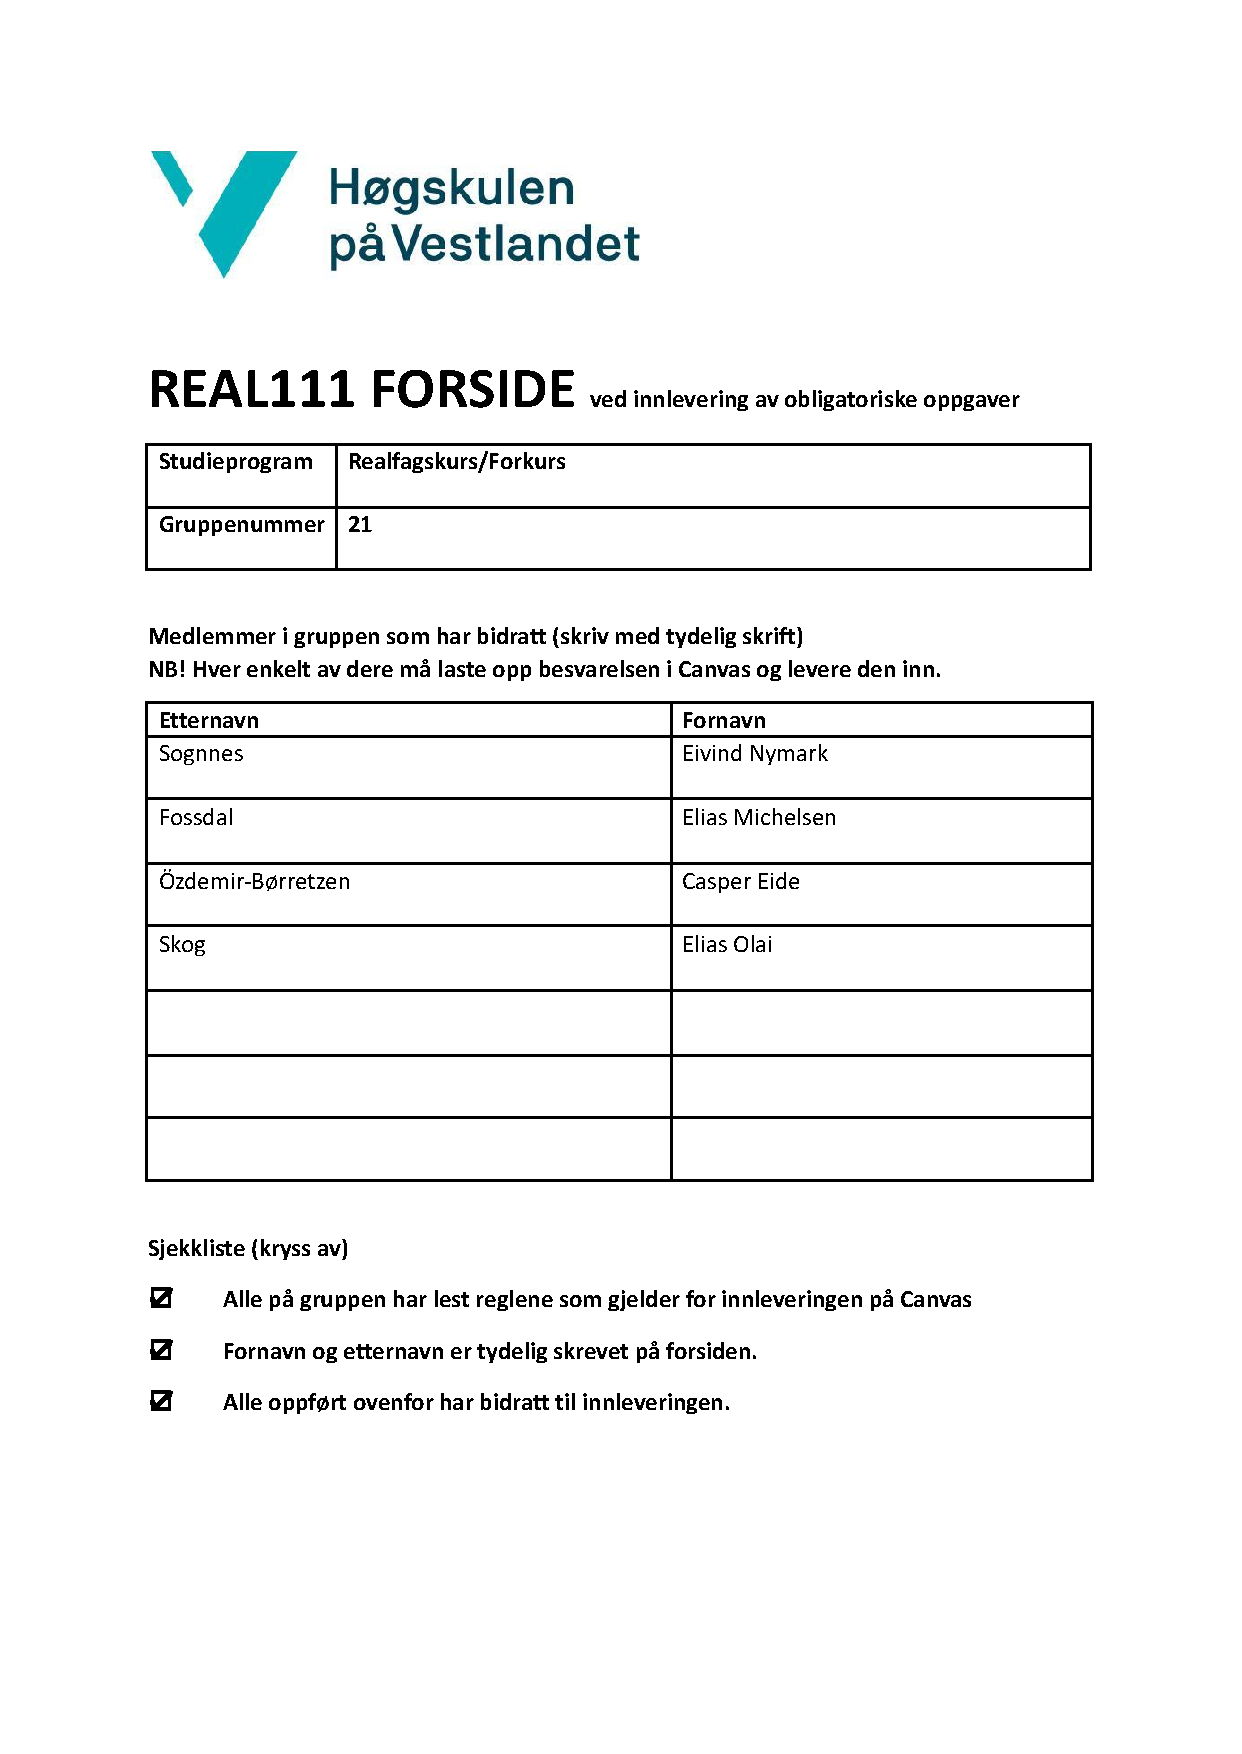
\includepdf[pages={1}]{real111-forside.pdf}

% % % % % % % % % % % % % % % % % % % % % % % % % % % % % % % % % % % % % % % % 

\section*{Laboratorierapport 2 av 2: Elektrolyse av vann}
Gruppe: Eivind N. Sognnes, Elias Fossdal, Casper Eide Özdemir-Børretzen, Elias Olai Skog

\subsection*{Innledning}
I denne laboratorieøvelsen skal vi gjennomføre elektrolyse av vann. Vi skal bruke elektrisk energi for å spalte vannmolekyler til ioner. Hensikten med øvelsen er å danne hydrogengass.\\\\
Vann tilføres en trehalskolbe, og elektristet tilsettes med positiv og negativ leder i hver sin side-hals. Side-halsen med positiv elektrode kalles anode. Her vil det skje en sur reaksjon og det vil dannes oksygengass. Side-halsen med negative elektrode kalles katode. Her vil det skje en basisk reaksjon og dannelse av hydrogengass.\\

\begin{center}
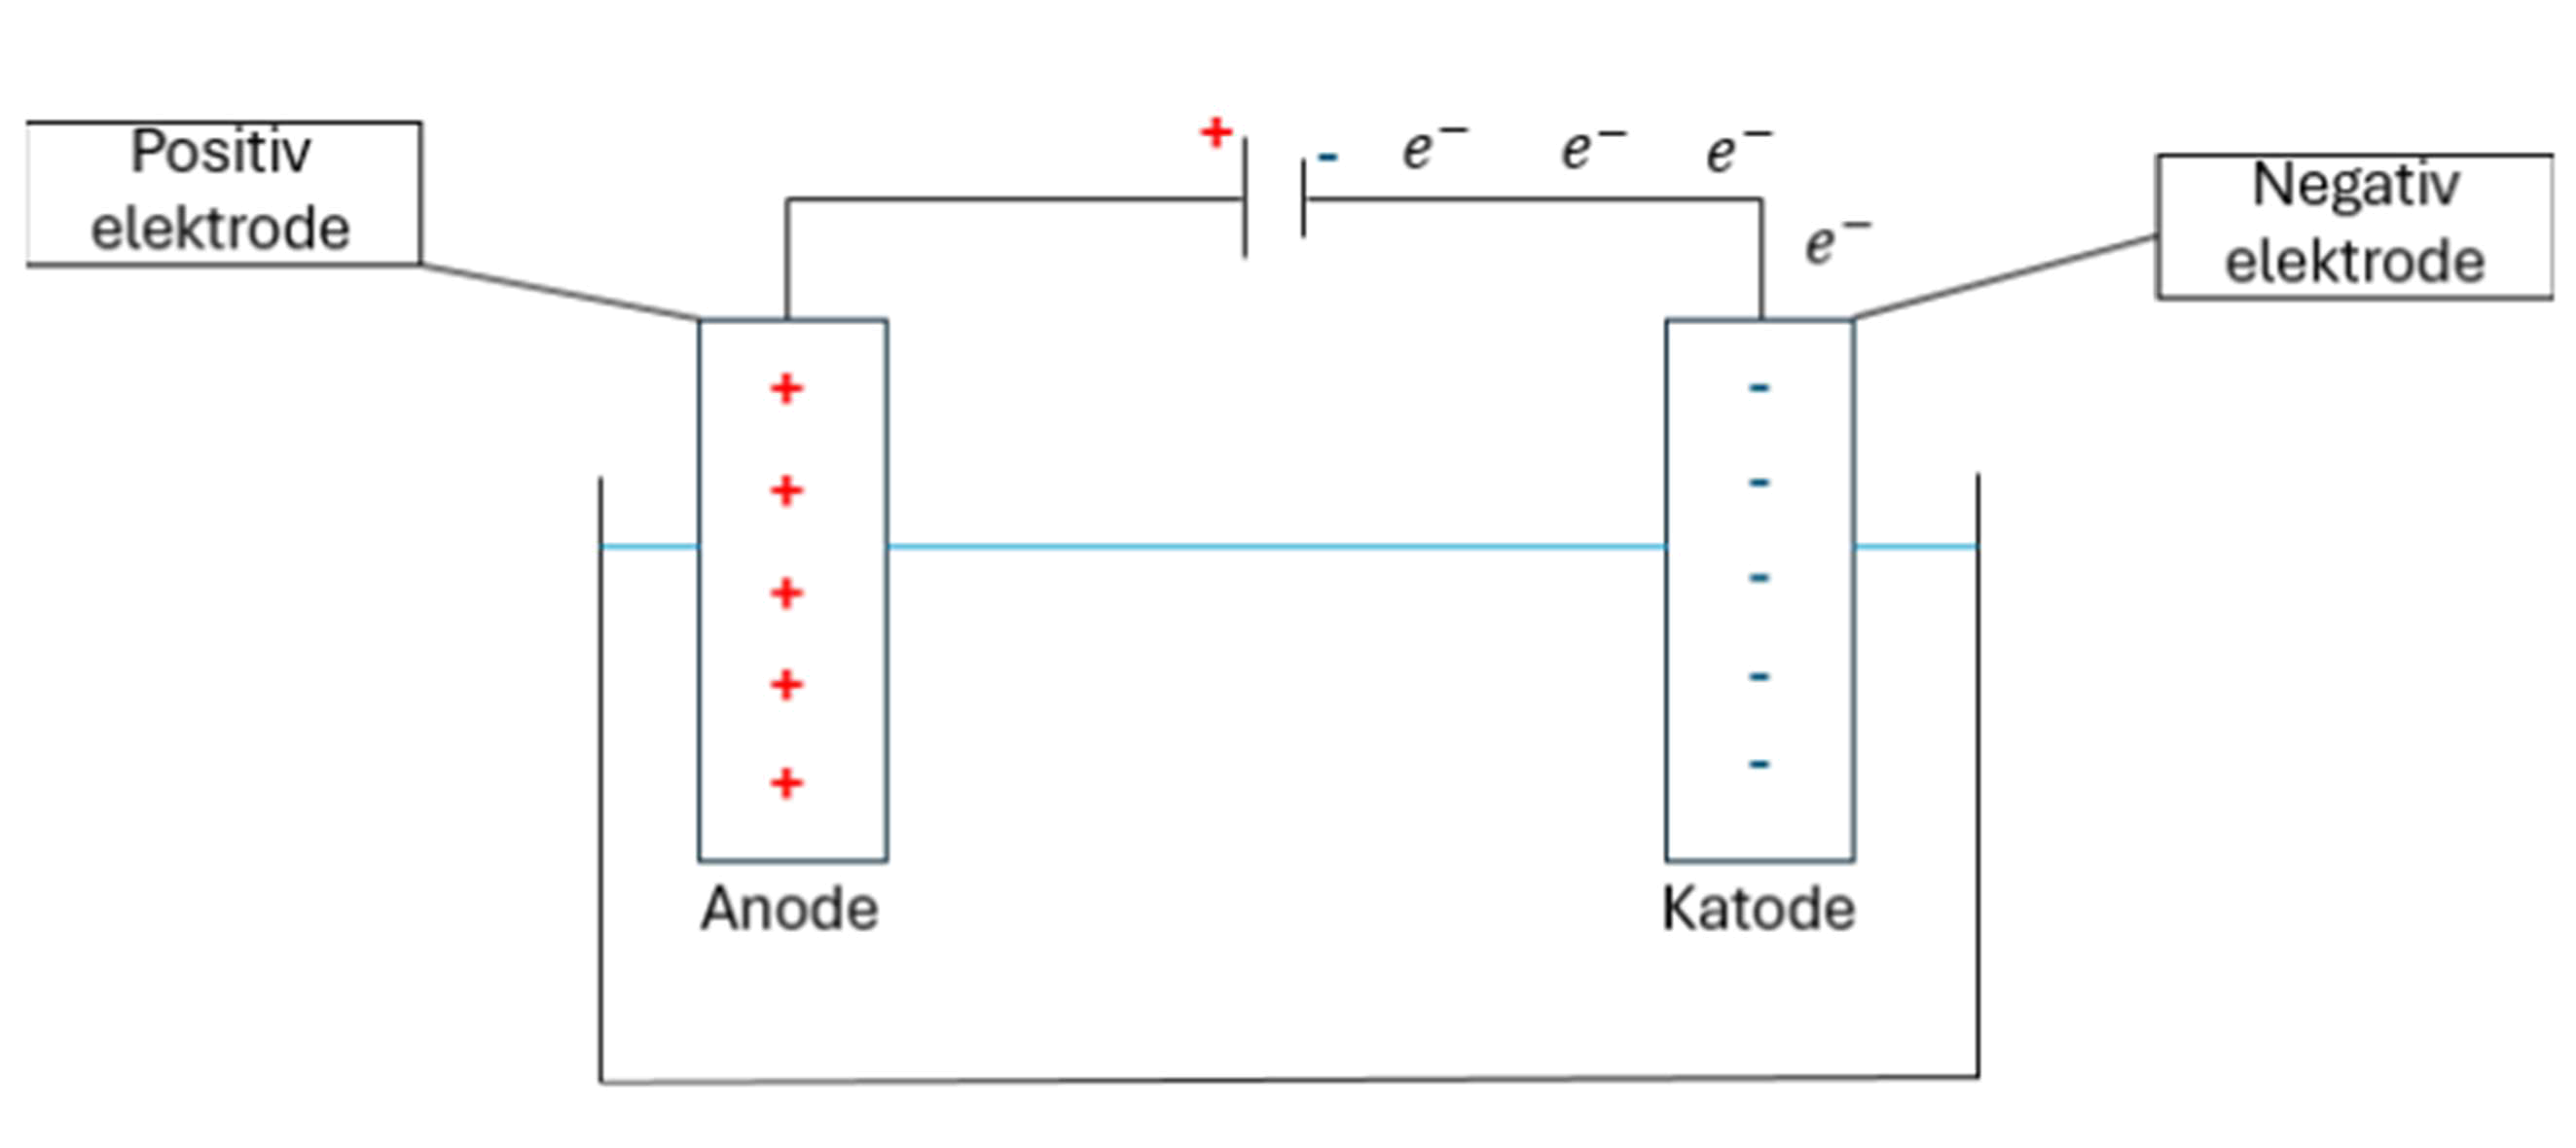
\includegraphics[scale=0.5]{elektrolyse1.png}
\end{center}

Natriumsulfat ($Na_2SO_4$) brukes i stedet for vann for å få en hurtigere reaksjon og bromtymolblått ($BTB$) blandes inn som indikator. $BTB$ er grønn i nøytral løsning ved $pH$-verdi $6,8$ og har fargeomslag til gult ved sur løsning og til blått ved basisk løsning.

\subsection*{Resultater}

\begin{tabular}{ l l l l }
& Observasjoner & Nettoligning & $E^0 (V)$ \\\\

Anodereaksjon: & Væsken går fra grønn til gul,  & $2H_2O(l) \rightarrow O_2(g) + 4H^+(aq) + 4e^-$ & $-1,23$ \\ 
& som indikerer redusert\\
& $pH$-verdi (forsuring).\\
& Det utvikles cirka halve mengden\\
& gass av det som skjer på katoden.\\
& Gassen som dannes er oksygen.\\[0.8cm]

Katodereaksjon: & Væsken går fra grønn til blå, & $4H_2O(l) + 4e^- \rightarrow 2H_2(g) + 4OH^-(aq)$ & $-0,83$ \\
& som indikerer økt $pH$-verdi\\
& (basisk reaksjon).\\
& Det utvikles cirka dobbel mengde\\
& gass i forhold til ved anoden.\\
& Gassen som dannes er hydrogen.\\[0.8cm]

Totalreaksjon: & & $6H_2O(l) \rightarrow O_2(g) + 4H_2O(l) + 2H_2(g)$ &\\
& & $= 2H_2O(l) \rightarrow O_2(g) + 2H_2(g)$ &
\end{tabular}

\vspace{1cm}

\begin{center}
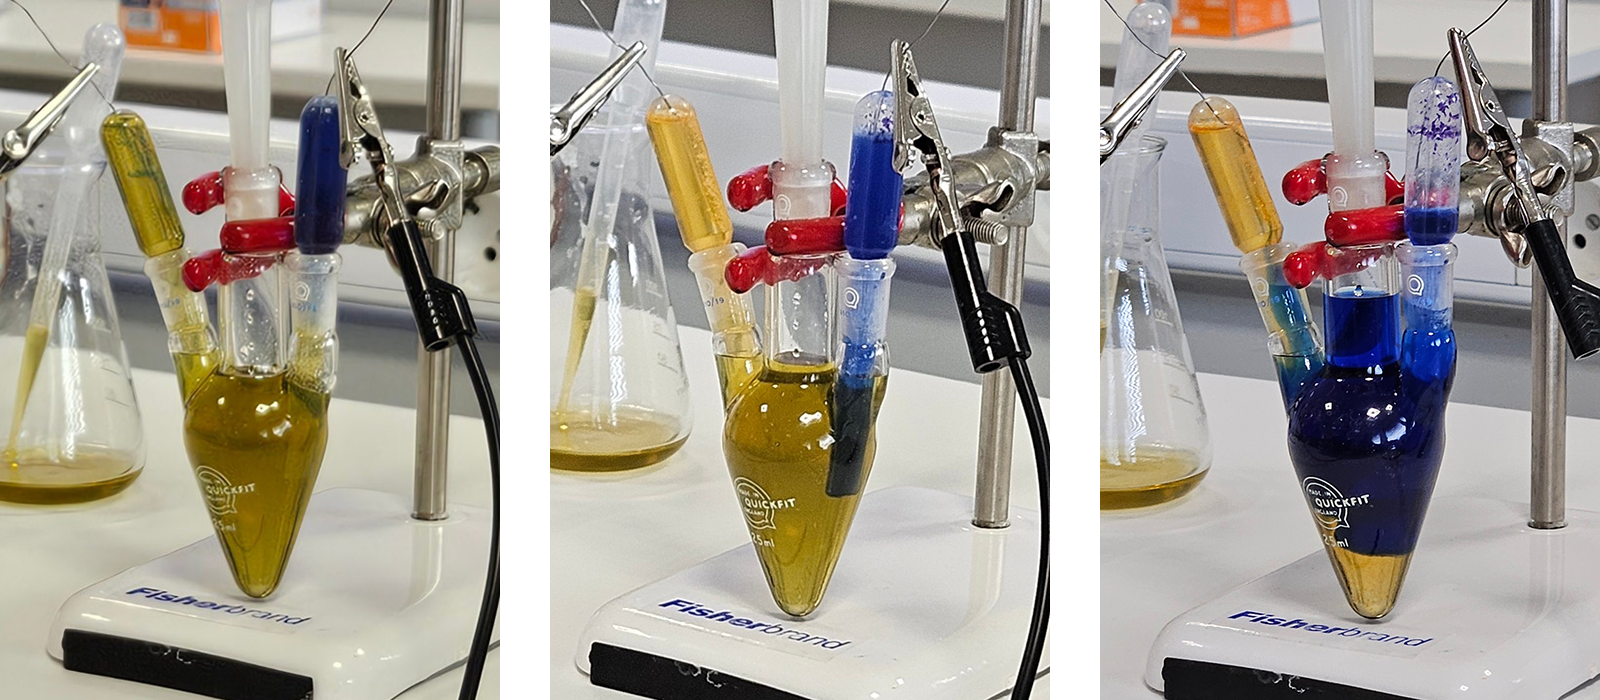
\includegraphics[scale=0.22]{resultat.png}
\end{center}

\vspace{1cm}

\begin{enumerate}[itemsep=1cm]
\item Den blå fargen ved katoden skyldes dannelse av hydroksidioner. Hvilken gass dannes ved katoden? Hvilken reaksjon skjer ved anoden?\\\\
Svar: Ved katoden dannes det hydrogengass. Ved anoden dannes det oksygengass.

\item BTB – Hva indikerer blå og gul farge?\\\\
Svar: Blåfarge i $BTB$ indikerer at væskens $pH$-verdi er over $6,8$ (basisk). Dersom $pH$-verdien er under $6,8$ (sur) er $BTB$ væsken gul. Dersom $BTB$ væsken er grønn vil det indikere at løsningen er nøytral.

\item Hvorfor tilsettes $Na_2SO_4$ til løsningen?\\\\
Svar: $Na_2SO_4$ benyttes siden saltet i væsken leder strømmen bedre enn i rent vann. Dette gir en vesentlig hurtigere kjemisk reaksjon.

\item Deltar $Na_2SO_4$ i reaksjonen?\\\\
Svar: Nei, stoffet deltar ikke direkte i reaksjonen men fungerer som en elektrolytt som leder strømmen.

\item Hvilken velkjent/berømt gassblanding får man om vi kombinerer gassproduktene fra elektrolyse av vann?\\\\
Svar: Da får man $2H_2O$. Dette er hydrogengass og oksygen med et 2:1 blandingsforhold. Dette er kjent som knallgass på grunn av at gassen er svært brennbar/eksplosiv.

\end{enumerate}

\subsection*{Konklusjon}
Vi tok i bruk spenningsrekken og huskeregelen ``Red Cat / An Ox'' for å beregne cellepotensialet for elektrolyse av vann. Øvelsen ble utført med forventet resultat, der vi kunne observere dannelse av oksygengass og hydrogengass i de to pipettene, samt fargeomslag i væskene. På bildene ser vi likevel at det dannes vesentlig mer oksygen enn hydrogen. Fra teorien forventet vi at det skulle dannes oksygen og hydrogen i forholdet 1:2. En feilkilde her er trolig at det ikke er helt tett mellom pipetten og anoden slik at noe av oksygengassen lekker ut her. 

% % % % % % % % % % % % % % % % % % % % % % % % % % % % % % % % % % % % % % % % 

\end{document}
